\documentclass[12pt]{article}
\usepackage[table]{xcolor}
\usepackage[shortlabels]{enumitem}
\usepackage{tabularx,xltabular}
\usepackage{graphicx}
\usepackage{hyperref}
\usepackage{verbatim}
\usepackage{geometry}
\usepackage{ulem}
\usepackage[official]{eurosym}
\usepackage{tikz}
\usetikzlibrary{arrows,backgrounds,calc,decorations.markings,patterns,3d}
\usepackage{pgfplots}
\pgfplotsset{compat = newest}
\usetikzlibrary{fit}
\newcommand\addvmargin[1]{
\usetikzlibrary{arrows}
\node[fit=(current bounding box),inner ysep=#1,inner xsep=0]{};}
\usepackage{cancel}
\usepackage{fontspec}
\usepackage{array}  
\geometry{a4paper, top=2cm, left=2cm, right=2cm, bottom=2cm, headsep=1cm}
\usepackage{tabu}
\usepackage{pst-node}
\usepackage{colortbl}
\usepackage{array}
\usepackage{german}
\setlength\parindent{0pt}
\newcolumntype{?}{!{\vrule width 1pt}}
\usepackage{makecell}
\renewcommand{\arraystretch}{2.5}
\usepackage{pbox}
\usepackage{amssymb}
\usepackage{amsmath}
\usepackage{booktabs}
\newcolumntype{L}[1]{>{\raggedright\let\newline\\\arraybackslash\hspace{0pt}}m{#1}}
\newcolumntype{C}[1]{>{\centering\let\newline\\\arraybackslash\hspace{0pt}}m{#1}}
\newcolumntype{R}[1]{>{\raggedleft\let\newline\\\arraybackslash\hspace{0pt}}m{#1}}
\begin{document}
\rightline{Datum: 14.06.2023}
\centerline{{\Large Tägliche Übungen}} 
\vspace{1cm}
\noindent \\


\begin{xltabular}{\textwidth}{|C{0.75cm}|X|}
\arrayrulecolor{black}\hline
a)&$4=x-50$
\\\hline
b)&$16=a+40$
\\\hline
c)&$9=y+34$
\\\hline
d)&$29=y-41$
\\\hline
e)&$12=y-34$
\\\hline
f)&$2=y-1$
\\\hline
g)&$1\cdot a+2\cdot a-4+1=12$
\\\hline
h)&$-1\cdot b+8+4\cdot b-24=17$
\\\hline
i)&$-3+2\cdot a-3+1\cdot a=3$
\\\hline
\end{xltabular}
\vspace{0.5cm}
\newpage
\rightline{Datum: 14.06.2023}
\centerline{{\large Lösungen Tägliche Übungen}} 
\vspace{0.5cm}

\begin{xltabular}{\textwidth}{|C{0.75cm}|X|}
\arrayrulecolor{black}\hline
a)&\begingroup\setlength{\jot}{-0.03cm}
\tikzstyle{background grid}=[draw, black!15,step=.5cm]
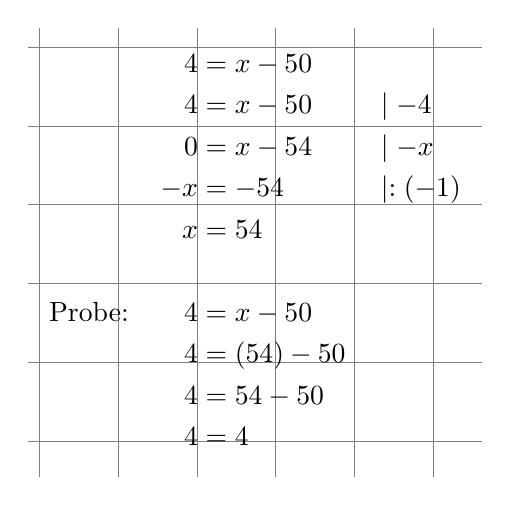
\begin{tikzpicture}[show background grid]
\node[below right] at (0,0.1) {
$\begin{aligned}
4 &=x-50& &  \\
4 &=x - 50& & \mid -4\\
0 &=x - 54& & \mid -x \\
-x &=-54& & \mid :\left(-1\right)\\
x &=54& & 
\\
\\
\mbox{Probe:}\qquad 4 &=x-50& &  \\
4 &=\left(54\right)-50& &  \\
4 &=54-50& &  \\
4 &=4& &  \\
\end{aligned}$};
\end{tikzpicture}
\endgroup
\\\hline
b)&\begingroup\setlength{\jot}{-0.03cm}
\tikzstyle{background grid}=[draw, black!15,step=.5cm]
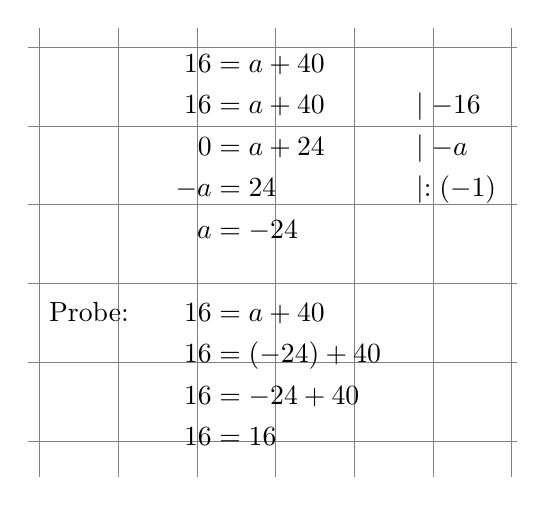
\begin{tikzpicture}[show background grid]
\node[below right] at (0,0.1) {
$\begin{aligned}
16 &=a+40& &  \\
16 &=a + 40& & \mid -16\\
0 &=a + 24& & \mid -a \\
-a &=24& & \mid :\left(-1\right)\\
a &=-24& & 
\\
\\
\mbox{Probe:}\qquad 16 &=a+40& &  \\
16 &=\left(-24\right)+40& &  \\
16 &=-24+40& &  \\
16 &=16& &  \\
\end{aligned}$};
\end{tikzpicture}
\endgroup
\\\hline
c)&\begingroup\setlength{\jot}{-0.03cm}
\tikzstyle{background grid}=[draw, black!15,step=.5cm]
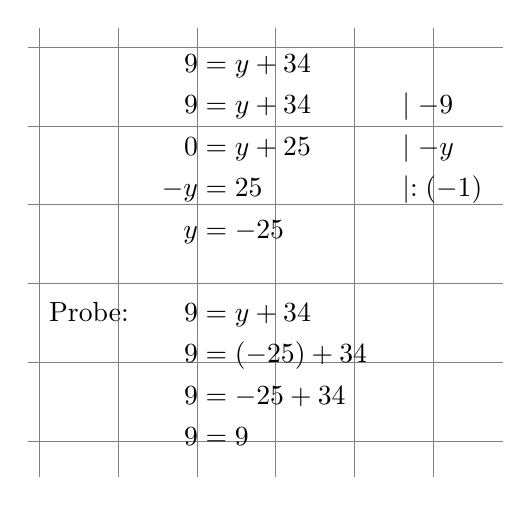
\begin{tikzpicture}[show background grid]
\node[below right] at (0,0.1) {
$\begin{aligned}
9 &=y+34& &  \\
9 &=y + 34& & \mid -9\\
0 &=y + 25& & \mid -y \\
-y &=25& & \mid :\left(-1\right)\\
y &=-25& & 
\\
\\
\mbox{Probe:}\qquad 9 &=y+34& &  \\
9 &=\left(-25\right)+34& &  \\
9 &=-25+34& &  \\
9 &=9& &  \\
\end{aligned}$};
\end{tikzpicture}
\endgroup
\\\hline
d)&\begingroup\setlength{\jot}{-0.03cm}
\tikzstyle{background grid}=[draw, black!15,step=.5cm]
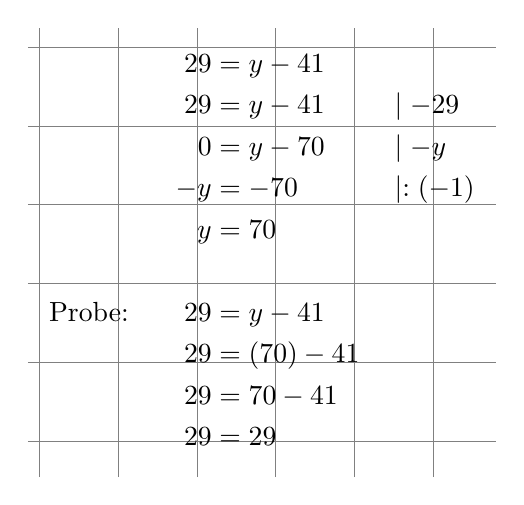
\begin{tikzpicture}[show background grid]
\node[below right] at (0,0.1) {
$\begin{aligned}
29 &=y-41& &  \\
29 &=y - 41& & \mid -29\\
0 &=y - 70& & \mid -y \\
-y &=-70& & \mid :\left(-1\right)\\
y &=70& & 
\\
\\
\mbox{Probe:}\qquad 29 &=y-41& &  \\
29 &=\left(70\right)-41& &  \\
29 &=70-41& &  \\
29 &=29& &  \\
\end{aligned}$};
\end{tikzpicture}
\endgroup
\\\hline
e)&\begingroup\setlength{\jot}{-0.03cm}
\tikzstyle{background grid}=[draw, black!15,step=.5cm]
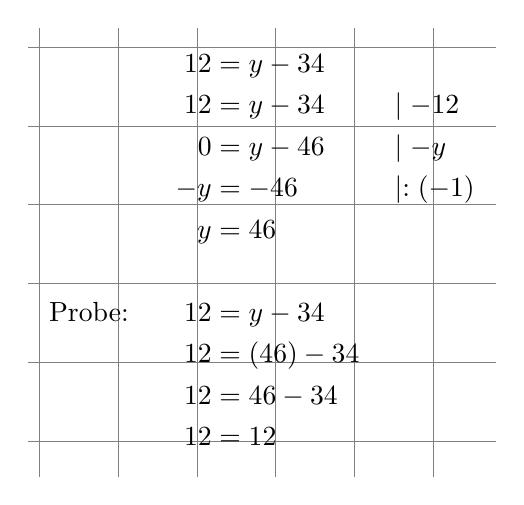
\begin{tikzpicture}[show background grid]
\node[below right] at (0,0.1) {
$\begin{aligned}
12 &=y-34& &  \\
12 &=y - 34& & \mid -12\\
0 &=y - 46& & \mid -y \\
-y &=-46& & \mid :\left(-1\right)\\
y &=46& & 
\\
\\
\mbox{Probe:}\qquad 12 &=y-34& &  \\
12 &=\left(46\right)-34& &  \\
12 &=46-34& &  \\
12 &=12& &  \\
\end{aligned}$};
\end{tikzpicture}
\endgroup
\\\hline
f)&\begingroup\setlength{\jot}{-0.03cm}
\tikzstyle{background grid}=[draw, black!15,step=.5cm]
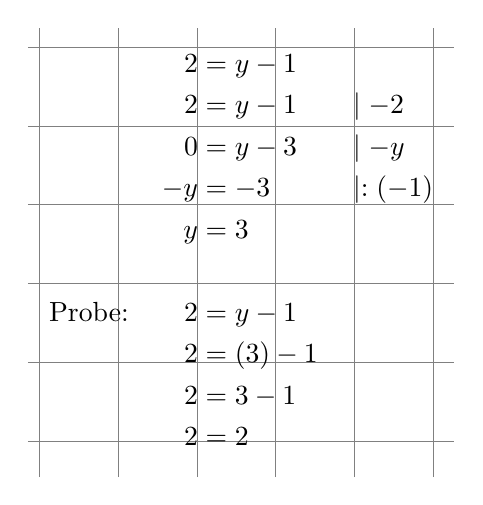
\begin{tikzpicture}[show background grid]
\node[below right] at (0,0.1) {
$\begin{aligned}
2 &=y-1& &  \\
2 &=y - 1& & \mid -2\\
0 &=y - 3& & \mid -y \\
-y &=-3& & \mid :\left(-1\right)\\
y &=3& & 
\\
\\
\mbox{Probe:}\qquad 2 &=y-1& &  \\
2 &=\left(3\right)-1& &  \\
2 &=3-1& &  \\
2 &=2& &  \\
\end{aligned}$};
\end{tikzpicture}
\endgroup
\\\hline
g)&\begingroup\setlength{\jot}{-0.03cm}
\tikzstyle{background grid}=[draw, black!15,step=.5cm]
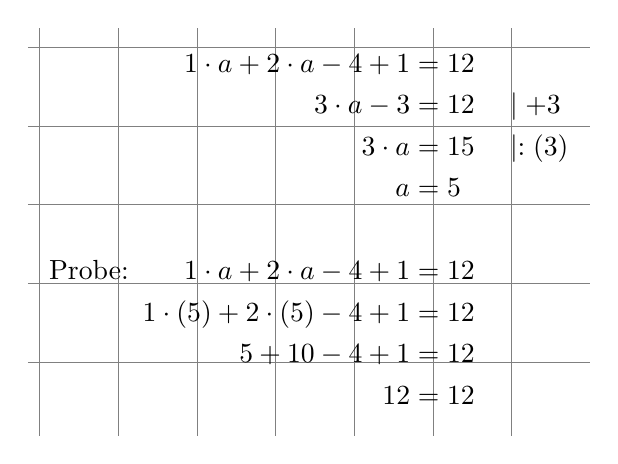
\begin{tikzpicture}[show background grid]
\node[below right] at (0,0.1) {
$\begin{aligned}
1\cdot a+2\cdot a-4+1 &=12& &  \\
3\cdot a - 3 &=12& & \mid + 3\\
3\cdot a &=15& & \mid :\left(3\right)\\
a &=5& & 
\\
\\
\mbox{Probe:}\qquad 1\cdot a+2\cdot a-4+1 &=12& &  \\
1\cdot \left(5\right)+2\cdot \left(5\right)-4+1 &=12& &  \\
5+10-4+1 &=12& &  \\
12 &=12& &  \\
\end{aligned}$};
\end{tikzpicture}
\endgroup
\\\hline
h)&\begingroup\setlength{\jot}{-0.03cm}
\tikzstyle{background grid}=[draw, black!15,step=.5cm]
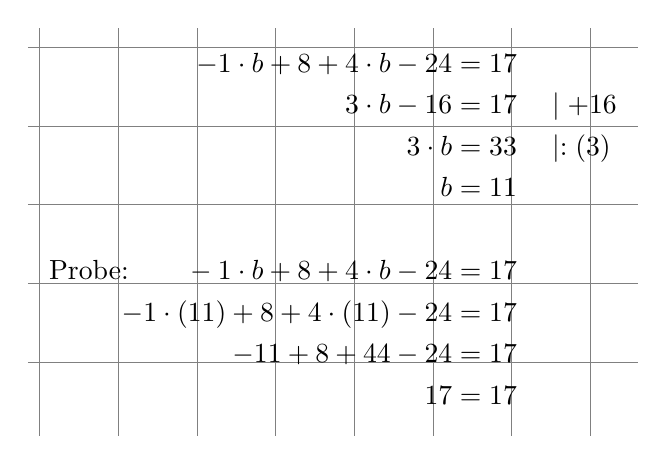
\begin{tikzpicture}[show background grid]
\node[below right] at (0,0.1) {
$\begin{aligned}
-1\cdot b+8+4\cdot b-24 &=17& &  \\
3\cdot b - 16 &=17& & \mid + 16\\
3\cdot b &=33& & \mid :\left(3\right)\\
b &=11& & 
\\
\\
\mbox{Probe:}\qquad -1\cdot b+8+4\cdot b-24 &=17& &  \\
-1\cdot \left(11\right)+8+4\cdot \left(11\right)-24 &=17& &  \\
-11+8+44-24 &=17& &  \\
17 &=17& &  \\
\end{aligned}$};
\end{tikzpicture}
\endgroup
\\\hline
i)&\begingroup\setlength{\jot}{-0.03cm}
\tikzstyle{background grid}=[draw, black!15,step=.5cm]
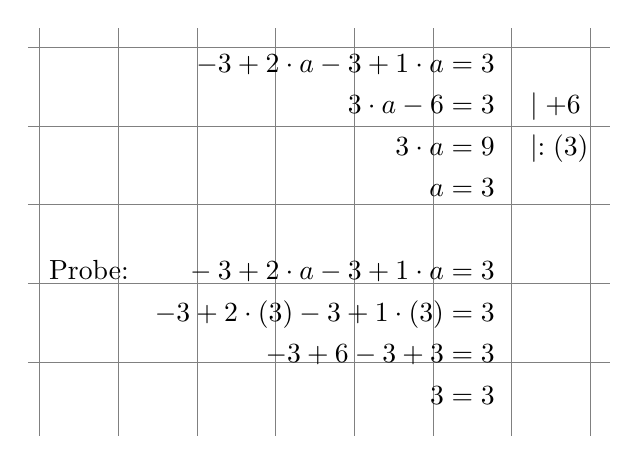
\begin{tikzpicture}[show background grid]
\node[below right] at (0,0.1) {
$\begin{aligned}
-3+2\cdot a-3+1\cdot a &=3& &  \\
3\cdot a - 6 &=3& & \mid + 6\\
3\cdot a &=9& & \mid :\left(3\right)\\
a &=3& & 
\\
\\
\mbox{Probe:}\qquad -3+2\cdot a-3+1\cdot a &=3& &  \\
-3+2\cdot \left(3\right)-3+1\cdot \left(3\right) &=3& &  \\
-3+6-3+3 &=3& &  \\
3 &=3& &  \\
\end{aligned}$};
\end{tikzpicture}
\endgroup
\\\hline
\end{xltabular}
\vspace{0.5cm}
\end{document}